% !TEX program = xelatex
\documentclass[11pt,a4paper]{article}

\usepackage[margin=1.8cm]{geometry}
\usepackage{fontspec}
\usepackage{xcolor}
\usepackage{graphicx}
\usepackage{tikz}
\usepackage{enumitem}
\usepackage{xcolor}

\definecolor{ink}{HTML}{1A1A1A}
\definecolor{mute}{HTML}{5C5C5C}
\definecolor{line}{HTML}{E6E6E6}
\definecolor{paper}{HTML}{FAFAFA}

% Shared light base (what Sophie asked: white / very light gray / very dark text)
\definecolor{baseWhite}{HTML}{FFFFFF}
\definecolor{baseWash}{HTML}{F5F5F5}
\definecolor{baseText}{HTML}{1F1F1F}
\definecolor{baseMuted}{HTML}{4A4A4A}
\definecolor{baseLine}{HTML}{E8E8E8}

% Palette accents
\definecolor{p1a}{HTML}{1F1F1F}
\definecolor{p1b}{HTML}{6B6B6B}
\definecolor{p1c}{HTML}{F5F5F5}
\definecolor{p1d}{HTML}{FFFFFF}

\definecolor{p2a}{HTML}{1C1917}
\definecolor{p2b}{HTML}{78716C}
\definecolor{p2c}{HTML}{A8A29E}
\definecolor{p2d}{HTML}{FAFAF9}

\definecolor{p3a}{HTML}{1E293B}
\definecolor{p3b}{HTML}{64748B}
\definecolor{p3c}{HTML}{CBD5E1}
\definecolor{p3d}{HTML}{F8FAFC}

\definecolor{p4a}{HTML}{1C1917}
\definecolor{p4b}{HTML}{9A3412}
\definecolor{p4c}{HTML}{E7E5E4}
\definecolor{p4d}{HTML}{FAFAF9}

\definecolor{p5a}{HTML}{14532D}
\definecolor{p5b}{HTML}{3F6212}
\definecolor{p5c}{HTML}{ECFCCB}
\definecolor{p5d}{HTML}{F7FEE7}

\definecolor{p6a}{HTML}{1E1B4B}
\definecolor{p6b}{HTML}{4338CA}
\definecolor{p6c}{HTML}{E0E7FF}
\definecolor{p6d}{HTML}{F8FAFC}

\definecolor{p7a}{HTML}{3B0764}
\definecolor{p7b}{HTML}{86198F}
\definecolor{p7c}{HTML}{FAE8FF}
\definecolor{p7d}{HTML}{FDF4FF}

\definecolor{p8a}{HTML}{134E4A}
\definecolor{p8b}{HTML}{0F766E}
\definecolor{p8c}{HTML}{CCFBF1}
\definecolor{p8d}{HTML}{F0FDFA}

\definecolor{p9a}{HTML}{111827}
\definecolor{p9b}{HTML}{B45309}
\definecolor{p9c}{HTML}{F5F5F4}
\definecolor{p9d}{HTML}{FFFFFF}

\definecolor{p10a}{HTML}{18181B}
\definecolor{p10b}{HTML}{BE123C}
\definecolor{p10c}{HTML}{F4F4F5}
\definecolor{p10d}{HTML}{FFFFFF}

\definecolor{p11a}{HTML}{0C0A09}
\definecolor{p11b}{HTML}{44403C}
\definecolor{p11c}{HTML}{D6D3D1}
\definecolor{p11d}{HTML}{FAFAF9}

\definecolor{p12a}{HTML}{172554}
\definecolor{p12b}{HTML}{1D4ED8}
\definecolor{p12c}{HTML}{DBEAFE}
\definecolor{p12d}{HTML}{F8FAFC}

\setmainfont{TeX Gyre Pagella}
\setsansfont{Montserrat}

\newcommand{\chiikologo}{%
  
\includegraphics[height=1.35cm]{../../public/chiikologosophie.png}%
}

\newcommand{\docheader}[1]{%
  \noindent
  \begin{tikzpicture}
    \fill[paper] (0,0) rectangle (\textwidth,2.1);
    \node[anchor=west] at (0.2,1.05) {\chiikologo};
    \node[anchor=east, align=right, text=ink] at (\textwidth-0.2,1.35) {%
      {\sffamily\bfseries\large Sophie Gomez --- Propuestas}\\[2pt]
      {\sffamily\color{mute}\small #1}\\[1pt]
      {\sffamily\color{mute}\footnotesize Chiiko · Documento de selección}
    };
  \end{tikzpicture}
  \vspace{0.35cm}
  {\color{line}\hrule height 0.6pt}
  \vspace{0.55cm}
}

\newcommand{\swatch}[2]{%
  \begin{tikzpicture}
    \fill[#1] (0,0) rectangle (1.55,1.15);
    \draw[line, line width=0.5pt] (0,0) rectangle (1.55,1.15);
    \node[anchor=north, font=\sffamily\fontsize{5.5}{6.5}\selectfont, text=mute] at (0.775,-0.08) {#2};
  \end{tikzpicture}%
}

\newcommand{\palettecard}[8]{%
  % #1 code, #2 name, #3 vibe, #4-#7 colors, #8 hex labels as one text line note
  \noindent
  \begin{tikzpicture}
    \draw[line, line width=0.7pt, fill=white] (0,0) rectangle (\textwidth,5.15);
    % mock browser bar
    \fill[#7] (0.25,2.55) rectangle (\textwidth-0.25,4.85);
    \draw[line, line width=0.5pt] (0.25,2.55) rectangle (\textwidth-0.25,4.85);
    \fill[#6] (0.25,4.35) rectangle (\textwidth-0.25,4.85);
    \node[anchor=west, font=\sffamily\bfseries\fontsize{8}{9}\selectfont, text=#4] at (0.45,4.6) {SOPHIE GOMEZ};
    \node[anchor=east, font=\sffamily\fontsize{6.5}{7.5}\selectfont, text=#5] at (\textwidth-0.45,4.6) {FR / ES / EN · Menu};
    \node[anchor=west, font=\sffamily\bfseries\fontsize{16}{18}\selectfont, text=#4] at (0.5,3.7) {SOPHIE GOMEZ};
    \node[anchor=west, font=\sffamily\fontsize{7.5}{9}\selectfont, text=#5] at (0.5,3.2) {Actrice · Modèle · Présence};
    \fill[#4] (0.5,2.75) rectangle (2.35,3.0);
    \node[anchor=center, font=\sffamily\fontsize{5.5}{6.5}\selectfont, text=#7] at (1.425,2.875) {BOOK ACTRICE};
    \draw[#4, line width=0.7pt] (2.55,2.75) rectangle (4.4,3.0);
    \node[anchor=center, font=\sffamily\fontsize{5.5}{6.5}\selectfont, text=#4] at (3.475,2.875) {BOOK MODÈLE};

    \node[anchor=north west, font=\sffamily\bfseries\small, text=ink] at (0.3,2.3) {#1 · #2};
    \node[anchor=north east, font=\sffamily\scriptsize, text=mute] at (\textwidth-0.3,2.3) {#3};
    \node[anchor=north west] at (0.3,1.85) {\swatch{#4}{Texto / fuerte}};
    \node[anchor=north west] at (2.05,1.85) {\swatch{#5}{Secundario}};
    \node[anchor=north west] at (3.8,1.85) {\swatch{#6}{Lavado / UI}};
    \node[anchor=north west] at (5.55,1.85) {\swatch{#7}{Fondo}};
    \node[anchor=south west, font=\sffamily\fontsize{6.5}{8}\selectfont, text=mute, text width=\textwidth-0.7cm] at (0.3,0.2) {#8};
  \end{tikzpicture}
  \vspace{0.28cm}
}

\pagestyle{empty}
\setlength{\parindent}{0pt}

\begin{document}
\color{ink}

\docheader{03 · Paletas de color (base clara)}

{\sffamily
\textbf{Punto de partida}\\[4pt]
{\color{mute}
Tomamos como base una dirección \textbf{clara}: fondo blanco o gris muy claro
y texto gris muy oscuro (casi negro). Es una buena base para que las fotos
y el contenido se lean con calma, y para mantener un look editorial limpio.
Las propuestas de abajo \textbf{parten de esa base} y solo cambian el acento
o la temperatura del color, para que puedas elegir sin perder esa claridad.
}
}

\vspace{0.35cm}

\section*{{\sffamily Base común (compartida en todas las propuestas)}}

\noindent
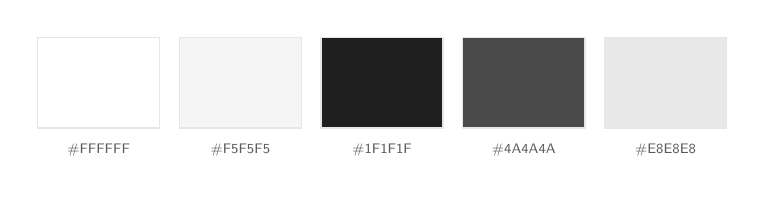
\begin{tikzpicture}
  \node at (0.8,0.7) {\swatch{baseWhite}{\#FFFFFF}};
  \node at (2.6,0.7) {\swatch{baseWash}{\#F5F5F5}};
  \node at (4.4,0.7) {\swatch{baseText}{\#1F1F1F}};
  \node at (6.2,0.7) {\swatch{baseMuted}{\#4A4A4A}};
  \node at (8.0,0.7) {\swatch{baseLine}{\#E8E8E8}};
\end{tikzpicture}

{\sffamily\color{mute}\footnotesize
Blanco · Gris lavado · Texto casi negro · Texto secundario · Líneas / bordes
}

\vspace{0.45cm}

\section*{{\sffamily Propuestas}}

\palettecard{P1}{Noir Paper}{Minimal absoluto}
{p1a}{p1b}{p1c}{p1d}
{Hex: \#1F1F1F · \#6B6B6B · \#F5F5F5 · \#FFFFFF --- Ideal si quieres máxima sobriedad casting/editorial.}

\palettecard{P2}{Stone Soft}{Cálida / piedra}
{p2a}{p2b}{p2c}{p2d}
{Hex: \#1C1917 · \#78716C · \#A8A29E · \#FAFAF9 --- Grises cálidos (stone). Menos ``hospital'', más papel.}

\palettecard{P3}{Slate Cool}{Fría / cine contemporáneo}
{p3a}{p3b}{p3c}{p3d}
{Hex: \#1E293B · \#64748B · \#CBD5E1 · \#F8FAFC --- Azul-gris frío. Muy fotográfico y digital.}

\newpage
\docheader{03 · Paletas de color (cont.)}

\palettecard{P4}{Terracotta Accent}{Acento tierra (1 color)}
{p4a}{p4b}{p4c}{p4d}
{Hex: \#1C1917 · \#9A3412 · \#E7E5E4 · \#FAFAF9 --- Base clara + un acento terracotta solo en CTAs/links.}

\palettecard{P5}{Olive Soft}{Acento natural}
{p5a}{p5b}{p5c}{p5d}
{Hex: \#14532D · \#3F6212 · \#ECFCCB · \#F7FEE7 --- Verde oliva suave. Sensación orgánica / editorial día.}

\palettecard{P6}{Ink Indigo}{Acento índigo sobrio}
{p6a}{p6b}{p6c}{p6d}
{Hex: \#1E1B4B · \#4338CA · \#E0E7FF · \#F8FAFC --- Índigo contenido (no ``purple AI''). Elegante y moderno.}

\palettecard{P7}{Plum Quiet}{Acento ciruela}
{p7a}{p7b}{p7c}{p7d}
{Hex: \#3B0764 · \#86198F · \#FAE8FF · \#FDF4FF --- Toque fashion; usar el acento con mucha moderación.}

\newpage
\docheader{03 · Paletas de color (cont.)}

\palettecard{P8}{Teal Archive}{Acento teal editorial}
{p8a}{p8b}{p8c}{p8d}
{Hex: \#134E4A · \#0F766E · \#CCFBF1 · \#F0FDFA --- Fresco, europeo, bueno para modelo + comunicación.}

\palettecard{P9}{Amber Signal}{Acento ámbar / CTA}
{p9a}{p9b}{p9c}{p9d}
{Hex: \#111827 · \#B45309 · \#F5F5F4 · \#FFFFFF --- Ámbar solo para botones. Alto contraste de acción.}

\palettecard{P10}{Rose Cinema}{Acento rosa cine}
{p10a}{p10b}{p10c}{p10d}
{Hex: \#18181B · \#BE123C · \#F4F4F5 · \#FFFFFF --- Rosa oscuro / berry. Dramático, memorable.}

\palettecard{P11}{Warm Graphite}{Sin color: solo grises cálidos}
{p11a}{p11b}{p11c}{p11d}
{Hex: \#0C0A09 · \#44403C · \#D6D3D1 · \#FAFAF9 --- Si prefieres cero acento de color: solo tipografía y foto.}

\newpage
\docheader{03 · Paletas de color (cont.)}

\palettecard{P12}{Navy Line}{Acento navy}
{p12a}{p12b}{p12c}{p12d}
{Hex: \#172554 · \#1D4ED8 · \#DBEAFE · \#F8FAFC --- Azul navy clásico. Confianza / agencia / Europa.}

\vspace{0.2cm}
\section*{{\sffamily Guía rápida Chiiko}}

{\sffamily\small
\begin{itemize}[leftmargin=1.1em, itemsep=0.18em]
  \item \textbf{Más casting / cine sobrio:} P1, P3, P11
  \item \textbf{Más moda / editorial:} P2, P4, P8
  \item \textbf{Más presencia de marca con 1 acento:} P4, P9, P10, P12
  \item \textbf{Evitar:} saturación alta en fondos enteros; el acento debe vivir en links/CTAs, no en toda la página.
\end{itemize}
}

\vspace{0.35cm}
\noindent
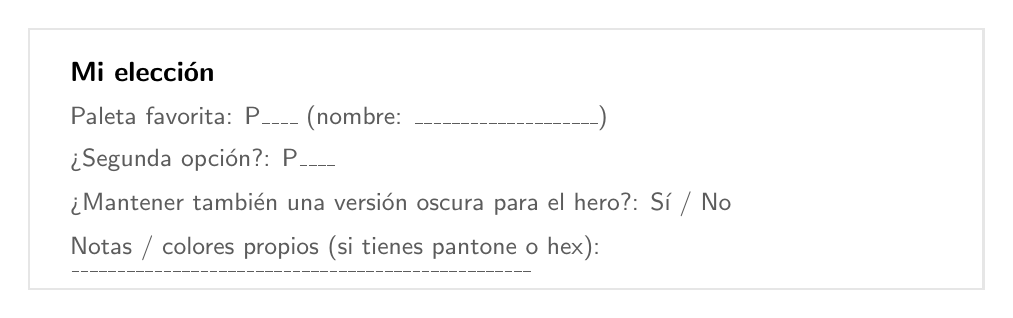
\begin{tikzpicture}
  \draw[line, line width=0.8pt] (0,0) rectangle (\textwidth,3.3);
  \node[anchor=north west, font=\sffamily\bfseries] at (0.4,3.0) {Mi elección};
  \node[anchor=north west, font=\sffamily\small, text=mute] at (0.4,2.45) {Paleta favorita: P\_\_\_\_  (nombre: \_\_\_\_\_\_\_\_\_\_\_\_\_\_\_\_\_\_\_\_)};
  \node[anchor=north west, font=\sffamily\small, text=mute] at (0.4,1.9) {¿Segunda opción?: P\_\_\_\_};
  \node[anchor=north west, font=\sffamily\small, text=mute] at (0.4,1.35) {¿Mantener también una versión oscura para el hero?:  Sí / No};
  \node[anchor=north west, font=\sffamily\small, text=mute] at (0.4,0.8) {Notas / colores propios (si tienes pantone o hex):};
  \node[anchor=north west, font=\sffamily\small, text=mute] at (0.4,0.35) {\_\_\_\_\_\_\_\_\_\_\_\_\_\_\_\_\_\_\_\_\_\_\_\_\_\_\_\_\_\_\_\_\_\_\_\_\_\_\_\_\_\_\_\_\_\_\_\_\_\_};
\end{tikzpicture}

\vspace{0.7cm}
{\sffamily\color{mute}\footnotesize
Chiiko · Propuestas de paleta para Sophie Gomez · Base clara solicitada (blanco / gris claro / texto oscuro)
}

\end{document}
